\documentclass{beamer}
\usecolortheme{beaver}
\beamertemplatenavigationsymbolsempty

% Fonts
\usepackage{fontspec}
\setmainfont{Source Serif Pro}[Ligatures=TeX]
\setsansfont{Source Sans Pro}[Ligatures=TeX]
\setmonofont{Source Code Pro}[
  BoldFont={* Medium},
  BoldItalicFont={* Medium Italic},
]

\usepackage[outputdir=out]{minted}
\usepackage{tikz}
\usetikzlibrary{positioning, fit}

\tikzset{
  invisible/.style={opacity=0,text opacity=0},
  highlight/.style={color=red},
  intro/.code args={<#1>}{%
    \only<#1>{\pgfkeysalso{highlight}}
    \alt<#1->{}{\pgfkeysalso{invisible}}
  },
}

\title{Rust MIR interpreter}
\author{
  Scott Olson
  \texorpdfstring{\\ \scriptsize{Supervisor: Christopher Dutchyn}}{}
}
\institute{
  CMPT 400 \\
  University of Saskatchewan
}
\date{}
\titlegraphic{
  
\includegraphics[width=64px,height=64px]{rust-logo-512x512.png} \\
  \scriptsize{\url{https://www.rust-lang.org}}
}

\begin{document}

\maketitle

\begin{frame}[fragile]
  \frametitle{What is Rust?}

  According to the website\dots

  \begin{quote}
    \textbf{Rust} is a systems programming language that runs blazingly fast,
    prevents nearly all segfaults, and guarantees thread safety.
  \end{quote}

  It's a new programming language from Mozilla, and it looks like this:

  \begin{minted}[
    autogobble,
    fontsize=\footnotesize,
    mathescape,
    xleftmargin=.3in,
  ]{rust}
    fn factorial(n: u64) -> u64 {
        (1..n).fold(1, |a, b| a * b)
    }

    fn main() {
        for x in 1..6 {
            println!("{}", factorial(x));
        }
        // $\Rightarrow$ 1
        // $\Rightarrow$ 1
        // $\Rightarrow$ 2
        // $\Rightarrow$ 6
        // $\Rightarrow$ 24
    }
  \end{minted}
\end{frame}

\begin{frame}
  \frametitle{How does Rust compile code?}

  \begin{center}
    \begin{tikzpicture}[x=4cm, y=3.5cm, auto, rounded corners]
      \tikzstyle{basic-stage}=[rectangle, draw, thick, align=center]
      \tikzstyle{stage}=[basic-stage, font=\tiny]
      \tikzstyle{pass}=[thick, -stealth]
      \tikzstyle{pass-label}=[font=\footnotesize]

      \node[basic-stage] (src) at (0,0) {Source\\Code};
      \node[basic-stage] (mach) at (2,-1) {Machine\\Code};

      \draw<1>[pass, out=0, in=180]
        (src.east) to node[font=\Huge] {?} (mach.west);

      \node[stage, intro=<2>] (ast) at (1,0)
        {\normalsize{AST} \\ Abstract Syntax Tree};
      \draw[pass, intro=<2>]
        (src) -- node[pass-label] {Parse} (ast);

      \node[stage, intro=<3>] (hir) at (2,0)
        {\normalsize{HIR} \\ High-level Intermediate\\Representation};
      \draw[pass, intro=<3>]
        (ast) -- node[pass-label] {Simplify} (hir);

      \node[stage, intro=<4>] (mir) at (0,-1)
        {\normalsize{MIR} \\ Mid-level Intermediate\\Representation};
      \path (hir.south) -- coordinate (middle) (mir.north);
      \draw[pass, intro=<4>]
        (hir.south) |- (middle) -| (mir.north);
      \node[pass-label, above, intro=<4>] at (middle) {Lower};

      \node[stage, intro=<5>] (llvm) at (1,-1)
        {\normalsize{LLVM IR} \\ Low-level Intermediate\\Representation};
      \draw[pass, intro=<5>]
        (mir) -- node[pass-label] {Translate} (llvm);

      \draw<6->[pass, intro=<6>]
        (llvm) -- node[pass-label] {Magic} (mach);

      \node[circle, draw, thick, intro=<7>, fit=(mir)] (focus) {};
      \node[intro=<7>, below] at (focus.south) {My focus};
    \end{tikzpicture}
  \end{center}
\end{frame}

\begin{frame}
  \frametitle{What is MIR?}

  \begin{itemize}
    \item \textbf{Problem:} Translating from the AST (or HIR) to LLVM IR is
      difficult and over-complicates the compiler.

    \item \textbf{MIR} is a simplified form of Rust that is well-suited for
      translation to LLVM IR.
  \end{itemize}
\end{frame}

\begin{frame}
  \frametitle{My project}

  \begin{itemize}
    \item But testing compiler passes can be difficult. How do we know that MIR
      does what we think it does?

      \begin{itemize}
        \item LLVM is very complicated and external to the Rust compiler!
      \end{itemize}
      \pause

    \item My project is to write an interpreter for MIR. Then we can check:
      \begin{equation*}
        \text{\parbox{3cm}{\centering Behaviour of\\ interpreted MIR}}
        =
        \text{\parbox{3cm}{\centering Behaviour of\\ compiled MIR}}
      \end{equation*}
  \end{itemize}
\end{frame}

\begin{frame}[fragile]
  \frametitle{MIR example}

  \begin{center}
    \begin{minted}{rust}
      fn square(n: u64) -> u64 {
        n * n
      }
    \end{minted}

    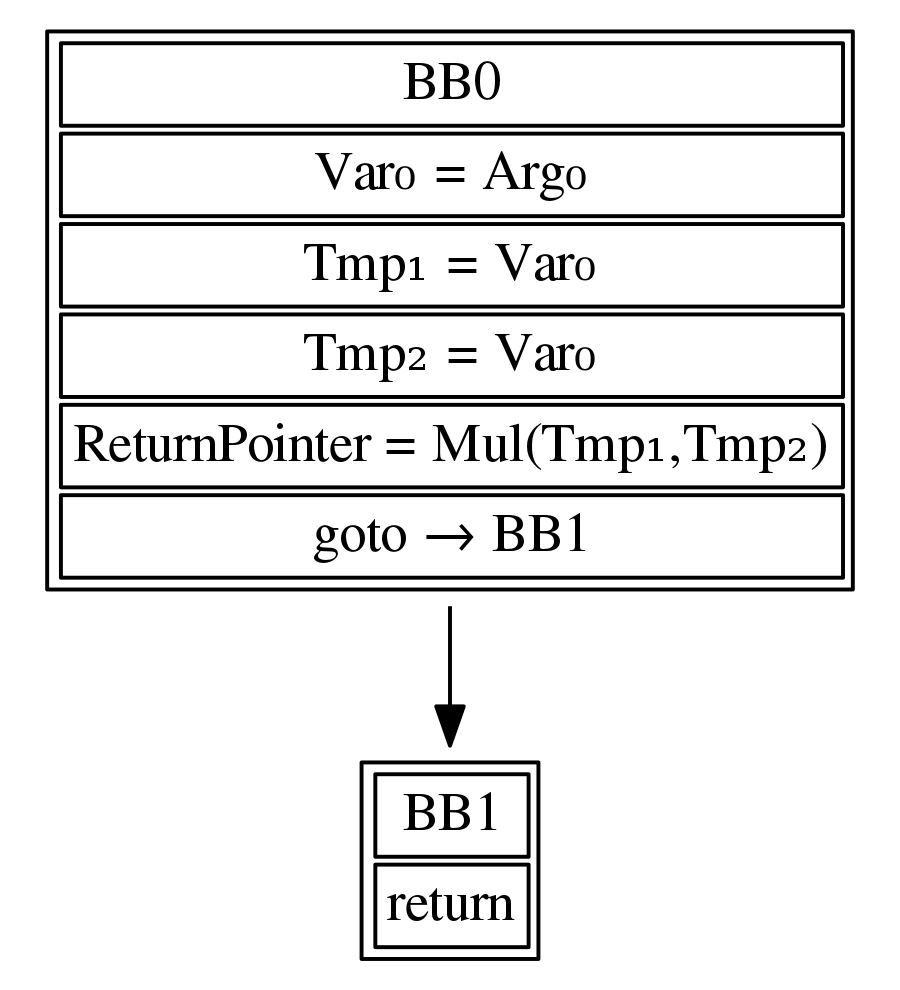
\includegraphics[width=140px]{mir-sample.png}
  \end{center}
\end{frame}

\begin{frame}
  \frametitle{Other possibilities}

  A MIR interpreter could be used for\dots

  \begin{itemize}
    \item unit testing the compiler (as mentioned)

    \item an interactive Rust command prompt \pause

    \item a GUI that steps through MIR execution one statement at a time

      \begin{itemize}
        \item for learning Rust, by seeing high-level code as MIR and tracing
          its execution

        \item for debugging
      \end{itemize}

      \pause

    \item executing code at compile-time for Rust's upcoming
      \mintinline{rust}{const fn} feature
  \end{itemize}
\end{frame}

\begin{frame}
  \begin{center}
    \LARGE{Questions?}
  \end{center}
\end{frame}

\end{document}
